% Standalone report: all diagrams and numerical figure data are embedded.
% Regenerate experiment data with report/scripts/reproduce.py.
\documentclass[11pt,a4paper]{article}
\usepackage[T1]{fontenc}
\usepackage{lmodern}
\usepackage[margin=24mm,top=22mm,bottom=23mm,headheight=14pt]{geometry}
\usepackage{amsmath,amssymb,booktabs,tabularx,array}
\usepackage{microtype,xcolor,graphicx,caption,float}
\usepackage{tikz,pgfplots}
\usetikzlibrary{arrows.meta,positioning,calc}
\pgfplotsset{compat=1.18}
\usepackage{enumitem,fancyhdr,listings,hyperref}
\definecolor{ink}{HTML}{163C53}
\definecolor{blue}{HTML}{216B99}
\definecolor{orange}{HTML}{BC621F}
\definecolor{muted}{HTML}{52636D}
\definecolor{pale}{HTML}{EDF3F6}
\definecolor{grid}{HTML}{D8E1E6}
\hypersetup{colorlinks=true,linkcolor=ink,citecolor=ink,urlcolor=ink,
 pdftitle={Poisson Reconstruction for Medical Imaging},
 pdfauthor={Yong-Hwan Lee and Tony Storey},
 pdfsubject={Expectation maximization and Fisher information in a nine-parameter tomography model}}
\pagestyle{fancy}
\fancyhf{}
\fancyhead[L]{\small\sffamily CT MEDICAL IMAGING}
\fancyhead[R]{\small\sffamily TECHNICAL REPORT}
\fancyfoot[L]{\small\sffamily Lee and Storey}
\fancyfoot[R]{\small\sffamily\thepage}
\renewcommand{\headrulewidth}{0pt}
\setlength{\parindent}{0pt}
\setlength{\parskip}{6pt}
\setlength{\emergencystretch}{2em}
\renewcommand{\arraystretch}{1.25}
\setlist{nosep,leftmargin=1.6em,topsep=4pt}
\captionsetup{font=small,labelfont=bf,justification=raggedright,singlelinecheck=false,skip=7pt}
\newcommand{\R}{\mathbb R}
\newcommand{\E}{\mathbb E}
\newcommand{\Pois}{\operatorname{Poisson}}
\newcommand{\diag}{\operatorname{diag}}
\newcommand{\tr}{\operatorname{tr}}
\newcommand{\ones}{\mathbf 1}
\newcommand{\sectionpage}[2]{\clearpage\section{#1}\label{#2}}
\newcommand{\smallnote}[1]{{\small\color{muted}#1\par}}
\lstset{basicstyle=\ttfamily\footnotesize,columns=fullflexible,keepspaces=true,
 showstringspaces=false,breaklines=true,frame=none,aboveskip=7pt,belowskip=7pt,
 keywordstyle=\bfseries\color{ink},commentstyle=\color{muted}}
\pgfplotsset{every axis/.append style={
 axis line style={grid},tick style={grid},
 tick label style={font=\small},label style={font=\small},
 legend style={font=\small,draw=none,fill=none},
 grid=major,grid style={grid!65},
 major tick length=2pt,minor tick num=0}}

\begin{document}
\thispagestyle{empty}
{\sffamily\small ECE565\quad ESTIMATION FILTERING AND DETECTION\par}
\vspace{12mm}
{\sffamily\bfseries\fontsize{31}{35}\selectfont
Poisson Reconstruction\\for Medical Imaging\par}
\vspace{5mm}
{\sffamily\large Expectation maximization and Fisher information\\
in a nine-parameter tomography model\par}
\vspace{7mm}
{\large Yong-Hwan Lee and Tony Storey\par}
\smallnote{Revised technical edition\quad 29 September 2026}
\vspace{9mm}

\textbf{Abstract}\par
Photon-counting inverse problems connect a physical measurement model to a statistical estimator. This report develops the linear Poisson model
$Y_i\sim\Pois((Ax)_i)$ for a $3\times3$ parameter field, derives its likelihood and Fisher information, and obtains a nonnegative expectation-maximization (EM) update from latent counts. The central distinction is between improving the likelihood of observed data and recovering the unknown field accurately: one does not guarantee the other.

The model is an educational tomography problem with emission-style additive intensities. It is not the exponential attenuation model of transmission X-ray CT. A controlled, seeded Monte Carlo study accompanies the derivation, with a fixed sensing matrix, explicit gain normalization, and a Cram\'er--Rao reference evaluated at the true parameters. These choices make the figures reproducible and keep numerical conclusions within the model actually simulated.

\vspace{5mm}
\begin{center}
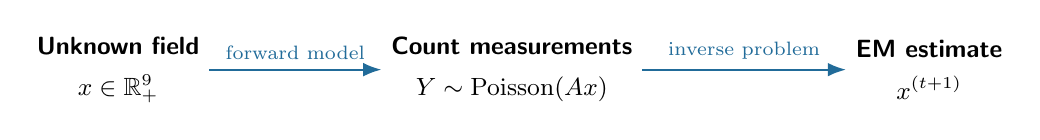
\begin{tikzpicture}[>=Latex,font=\sffamily\small]
 \node[align=center] (a) at (0,0) {\textbf{Unknown field}\\[4pt]$x\in\R_+^9$};
 \node[align=center] (b) at (5.0,0) {\textbf{Count measurements}\\[4pt]$Y\sim\Pois(Ax)$};
 \node[align=center] (c) at (10.3,0) {\textbf{EM estimate}\\[4pt]$x^{(t+1)}$};
 \draw[->,thick,blue] (a.east) -- node[above,font=\scriptsize]{forward model} (b.west);
 \draw[->,thick,blue] (b.east) -- node[above,font=\scriptsize]{inverse problem} (c.west);
\end{tikzpicture}
\end{center}
\vspace{4mm}
\textbf{What the study establishes}\par
Across 40\,000 simulated trials, the final EM error is approximately 17\% below that of the clipped least-squares initialization. Its gain-normalized MSE follows the Fisher-information reference within Monte Carlo uncertainty. A single-trial trace also shows error increasing during early likelihood ascent, demonstrating why data fit and reconstruction quality must be evaluated separately.

\vfill
{\small\sffamily
\begin{tabularx}{\linewidth}{@{}Xr@{}}
Measurement model and geometry & \pageref{sec:model}\\
Likelihood information and EM & \pageref{sec:likelihood}--\pageref{sec:em}\\
Controlled experiment and results & \pageref{sec:study}--\pageref{sec:convergence}\\
Implementation audit and reproducibility & \pageref{sec:audit}--\pageref{sec:reproduce}
\end{tabularx}}

\sectionpage{Measurement model and geometry}{sec:model}
\subsection*{The statistical model used here}
Let $A\in\R_+^{m\times n}$ be known, with $m=16$ measurements and $n=9$ unknown nonnegative intensities. Distinct observations are independent:
\begin{equation}
 Y_i\sim\Pois(\mu_i),\qquad \mu_i=(Ax)_i=\sum_{j=1}^n a_{ij}x_j.
 \label{eq:model}
\end{equation}
The binary weights used in this study indicate which pixels contribute to each observation. They are an idealized sensing design, not a calibrated scanner geometry. Full column rank, rather than a universal requirement for 16 rays, is the relevant identifiability condition for this linear mean model.

\begin{figure}[H]
\centering
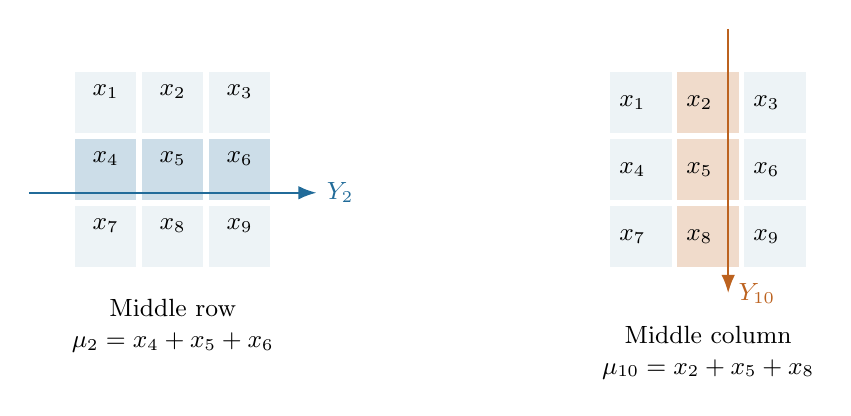
\begin{tikzpicture}[scale=0.85,>=Latex,font=\small]
\begin{scope}
 \fill[pale] (0,0) rectangle (3,3);
 \fill[blue!23] (0,1) rectangle (3,2);
 \draw[step=1cm,white,line width=2pt] (0,0) grid (3,3);
 \foreach \j/\x/\y in {1/.5/2.5,2/1.5/2.5,3/2.5/2.5,4/.5/1.5,5/1.5/1.5,6/2.5/1.5,7/.5/.5,8/1.5/.5,9/2.5/.5}
  \node at (\x,\y+.16) {$x_{\j}$};
 \draw[blue,thick,->] (-.65,1.15)--(3.65,1.15) node[right] {$Y_2$};
 \node[anchor=north,align=center] at (1.5,-.3) {Middle row\\$\mu_2=x_4+x_5+x_6$};
\end{scope}
\begin{scope}[xshift=8cm]
 \fill[pale] (0,0) rectangle (3,3);
 \fill[orange!23] (1,0) rectangle (2,3);
 \draw[step=1cm,white,line width=2pt] (0,0) grid (3,3);
 \foreach \j/\x/\y in {1/.5/2.5,2/1.5/2.5,3/2.5/2.5,4/.5/1.5,5/1.5/1.5,6/2.5/1.5,7/.5/.5,8/1.5/.5,9/2.5/.5}
  \node at (\x-.13,\y) {$x_{\j}$};
 \draw[orange,thick,->] (1.8,3.6)--(1.8,-.35) node[right] {$Y_{10}$};
 \node[anchor=north,align=center] at (1.5,-.7) {Middle column\\$\mu_{10}=x_2+x_5+x_8$};
\end{scope}
\end{tikzpicture}
\caption{Two rows of the fixed sensing matrix. The totals $Y_i$ are random counts; the sums shown are their expectations. Pixel indices run left to right, then top to bottom.}
\end{figure}

\subsection*{How this differs from transmission CT}
For an ideal monoenergetic transmission model, detected photons have mean
\begin{equation}
 \bar y_i=I_{0,i}\exp\!\left(-\sum_j l_{ij}\alpha_j\right)+r_i,
 \label{eq:transmission}
\end{equation}
where $\alpha_j$ is an attenuation coefficient, $l_{ij}$ a path length, $I_{0,i}$ an incident intensity, and $r_i$ a background mean. The exponential describes attenuation along the path~\cite{miqueles}. A logarithm can linearize the noiseless, background-free relation, but it does not preserve a Poisson distribution. Equation~\eqref{eq:model} is therefore analyzed on its own terms; $x_j$ is an intensity, not a physical CT attenuation coefficient. The additive construction is consistent with the mathematical structure used in emission reconstruction~\cite{shepp}.

\begin{table}[H]\small
\caption{Notation used consistently throughout the report.}
\begin{tabularx}{\linewidth}{@{}lXl@{}}\toprule
Symbol & Meaning & Dimension\\\midrule
$A$ & Known nonnegative sensing matrix & $16\times9$\\
$x$, $b$ & Intensity vector and fixed base vector, $x=gb$ & $9\times1$\\
$Y$, $y$, $\mu$ & Random counts, observed counts, and mean $Ax$ & $16\times1$\\
$N_{ij}$ & Unobserved contribution of pixel $j$ to count $i$ & Scalar\\
$g$, $t$, $R$ & Gain, iteration index, and Monte Carlo trial count & Scalars\\\bottomrule
\end{tabularx}
\end{table}

\sectionpage{Likelihood and statistical information}{sec:likelihood}
\subsection*{A constrained likelihood objective}
Given an observed count vector $y$, independence gives
\begin{align}
 L(x;y)&=\prod_{i=1}^m\frac{e^{-(Ax)_i}(Ax)_i^{y_i}}{y_i!},\\
 \ell(x;y)&=\sum_{i=1}^m\left[y_i\log(Ax)_i-(Ax)_i-\log\Gamma(y_i+1)\right].
 \label{eq:loglike}
\end{align}
The estimate maximizes $\ell$ over $x\geq0$. Use $0\log\mu=0$ for zero counts, including the continuous extension at $y_i=\mu_i=0$. A positive count with zero predicted mean has log likelihood $-\infty$. The likelihood itself is not set to zero to obtain an optimum; one uses the score in the interior or constrained optimality conditions on the boundary.

The generalized KL divergence, also called I-divergence, is
\begin{equation}
 D(y\Vert Ax)=\sum_i\left[y_i\log\frac{y_i}{(Ax)_i}-y_i+(Ax)_i\right].
\end{equation}
It differs from $-\ell(x;y)$ only by terms independent of $x$. Thus minimizing this divergence and maximizing the Poisson likelihood give the same solutions. The logarithm is of a ratio, not a ratio of logarithms. Neither vector needs to sum to one.

\subsection*{Fisher information and the Cram\'er--Rao reference}
At a point with positive means, the score and Hessian are
\begin{align}
 \nabla\ell(x)&=A^\mathsf T\!\left(\frac{y}{Ax}-\ones\right),\\
 \nabla^2\ell(x)&=-A^\mathsf T\diag\!\left(\frac{y_i}{(Ax)_i^2}\right)A.
\end{align}
Division in vector expressions is elementwise. Taking the expected negative Hessian yields
\begin{equation}
 \mathcal I_x(x)=A^\mathsf T\diag\!\left(\frac{1}{(Ax)_i}\right)A,
 \qquad \operatorname{Cov}(\widehat x)\succeq\mathcal I_x(x)^{-1}.
 \label{eq:fisher}
\end{equation}
The covariance inequality requires an unbiased estimator and the usual interior regularity conditions. Full column rank and positive means make $\mathcal I_x$ positive definite. A finite-iteration, nonnegative EM estimator may be biased; the ordinary CRLB is then a reference, not a universal lower bound on its MSE.

\subsection*{Why gain normalization changes the trend}
For $x=gb$ and fixed $A$, $\mathcal I_x(gb)=\mathcal I_x(b)/g$. Absolute variance in $x$ therefore has a reference proportional to $g$. Error on the base-intensity scale uses $\widehat b=\widehat x/g$ and has reference
\begin{equation}
 C_b(g)=\frac{1}{ng^2}\tr\!\left[\mathcal I_x(gb)^{-1}\right]
       =\frac{1}{ng}\tr\!\left[\mathcal I_x(b)^{-1}\right].
 \label{eq:gain}
\end{equation}
The expected $1/g$ decrease concerns this normalized error. Increasing an additive intensity is not equivalent to increasing an attenuation coefficient in Equation~\eqref{eq:transmission}.

\sectionpage{Expectation maximization}{sec:em}
\subsection*{Complete data and the E step}
Introduce independent latent variables $N_{ij}\sim\Pois(a_{ij}x_j)$ with $Y_i=\sum_jN_{ij}$. Conditional on the total, the vector of contributions is multinomial:
\begin{equation}
 (N_{i1},\ldots,N_{in})\mid Y_i=y_i,x^{(t)}
 \sim\operatorname{Multinomial}\!\left(y_i;\frac{a_{i1}x_1^{(t)}}{\mu_i^{(t)}},\ldots,
 \frac{a_{in}x_n^{(t)}}{\mu_i^{(t)}}\right).
\end{equation}
Its marginal conditional expectation is
\begin{equation}
 \widehat N_{ij}^{(t)}=\E[N_{ij}\mid y_i,x^{(t)}]
   =y_i\frac{a_{ij}x_j^{(t)}}{(Ax^{(t)})_i}.
\end{equation}
When $a_{ij}=0$, $N_{ij}=0$ almost surely; that term contributes zero. This is a superposition of Poisson counts, not a finite mixture distribution.

\subsection*{The M step and multiplicative update}
Dropping terms constant in $x$, the expected complete-data log likelihood separates by pixel:
\begin{align}
 Q(x\mid x^{(t)})&=\sum_{i,j}\left[\widehat N_{ij}^{(t)}\log(a_{ij}x_j)-a_{ij}x_j\right]+C,\\
 \frac{\partial Q}{\partial x_j}&=\frac{\sum_i\widehat N_{ij}^{(t)}}{x_j}-\sum_i a_{ij}.
\end{align}
Set the derivative to zero, with the boundary value zero if the expected total is zero. Writing $s=A^\mathsf T\ones$ gives
\begin{equation}
 \boxed{\quad x^{(t+1)}=x^{(t)}\odot
 \frac{A^\mathsf T\!\left(y/(Ax^{(t)})\right)}{A^\mathsf T\ones}\quad}
 \label{eq:em}
\end{equation}
Here $\odot$ denotes elementwise multiplication. With valid initialization and an exact M step, EM makes the observed likelihood nondecreasing~\cite{dempster}. This form is the classical multiplicative Poisson reconstruction update~\cite{shepp}.

\subsection*{A numerically explicit implementation}
\begin{lstlisting}[language=Matlab]
% A is m-by-n, y and x are column vectors; s > 0.
s = sum(A, 1)';
for t = 1:max_iter
    mu = A*x;
    assert(all(mu > 0 | y == 0));
    ratio = zeros(size(y));
    use = (mu > 0);
    ratio(use) = y(use)./mu(use);
    x_new = x .* (A'*ratio) ./ s;
    relative_change = norm(x_new-x)/max(norm(x), realmin);
    x = x_new;
end
\end{lstlisting}
Initialize every coordinate strictly positively: a zero coordinate is locked at zero by the multiplicative update. Check finite inputs, nonnegative weights and counts, nonzero column sensitivities, and likelihood ascent. For exact likelihood values, use \texttt{gammaln(y+1)}; no Stirling approximation is needed. The companion script implements the same update in batched NumPy form.

\sectionpage{Controlled numerical study}{sec:study}
The revised study fixes the geometry and underlying field so that another run can reproduce the comparison. It is a new synthetic verification experiment, separate from the unseeded legacy figures. No clinical images enter the estimator.

\begin{table}[H]\small
\caption{Experiment settings used for all reported numerical results.}
\begin{tabularx}{\linewidth}{@{}lX@{}}\toprule
Setting & Value\\\midrule
Sensing design & Predefined $16\times9$ matrix from \texttt{main.m}; rank 9\\
Base intensity $b^\mathsf T$ & $(120,240,360,180,720,300,90,420,540)$\\
Gain and observations & $g\in\{0.1,1,5,10\}$; $Y_i\sim\Pois((Agb)_i)$\\
Monte Carlo size & 10\,000 independent trials per gain; 40\,000 total\\
Random generator & NumPy PCG64; seed 20260929\\
Initialization & $x^{(0)}=\max(\operatorname{lstsq}(A,y),10^{-8})$ elementwise\\
Iteration budget & 1\,000 updates; checkpoints at 0, 20, 200 and 1\,000\\
Information reference & $\mathcal I_x(gb)$ evaluated at the true intensity $gb$\\\bottomrule
\end{tabularx}
\end{table}

\subsection*{Fixed geometry and field}
The matrix below is the one illustrated in Section~\ref{sec:model}. Its binary entries specify pixel membership; diagonal paths are not weighted by physical path length. The original script subsequently overwrites this matrix with a random one. That overwrite is deliberately excluded from the controlled study.
\begin{center}
\begin{minipage}[c]{0.56\linewidth}
\centering\small
\setlength{\arraycolsep}{3.5pt}
\renewcommand{\arraystretch}{1.02}
$A=\begin{bmatrix}
0&0&0&0&0&0&1&1&1\\
0&0&0&1&1&1&0&0&0\\
1&1&1&0&0&0&0&0&0\\
0&0&0&0&0&0&1&0&0\\
0&0&0&1&0&0&0&1&0\\
1&0&0&0&1&0&0&0&1\\
0&1&0&0&0&1&0&0&0\\
0&0&1&0&0&0&0&0&0\\
1&0&0&1&0&0&1&0&0\\
0&1&0&0&1&0&0&1&0\\
0&0&1&0&0&1&0&0&1\\
1&0&0&0&0&0&0&0&0\\
0&1&0&1&0&0&0&0&0\\
0&0&1&0&1&0&1&0&0\\
0&0&0&0&0&1&0&1&0\\
0&0&0&0&0&0&0&0&1
\end{bmatrix}$
\end{minipage}\hfill
\begin{minipage}[c]{0.40\linewidth}
\centering
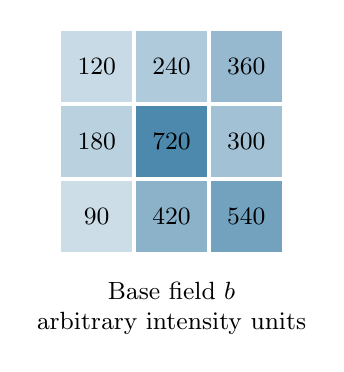
\begin{tikzpicture}[scale=.95,font=\small]
\foreach \v/\x/\y in {120/0/2,240/1/2,360/2/2,180/0/1,720/1/1,300/2/1,90/0/0,420/1/0,540/2/0}{
 \pgfmathtruncatemacro{\shade}{15+65*(\v/720)}
 \fill[blue!\shade!white] (\x,\y) rectangle +(1,1);
 \node at (\x+.5,\y+.5) {\v};
}
\draw[step=1cm,white,line width=1.2pt] (0,0) grid (3,3);
\node[anchor=north,align=center] at (1.5,-.25) {Base field $b$\\arbitrary intensity units};
\end{tikzpicture}
\end{minipage}
\end{center}

\subsection*{Error and simulation uncertainty}
For trial $r$, let $q_r(g,t)=\|x_r^{(t)}/g-b\|_2^2/n$. The reported MSE is $\bar q=R^{-1}\sum_rq_r$, and its Monte Carlo standard error is $s_q/\sqrt R$, with $s_q$ the sample standard deviation across independent trials. Approximate 95\% Monte Carlo intervals use $\bar q\pm1.96s_q/\sqrt R$. These quantify simulation uncertainty in the average error, not uncertainty in an individual reconstructed pixel.

% RESULTS_START
\sectionpage{Estimation error across signal gain}{sec:results}
The gain-normalized MSE falls as the photon intensity increases. At 1\,000 updates, EM reduces average error by approximately 17\% relative to its clipped least-squares initialization at each gain. The measured MSE-to-CRLB ratios range from 0.998 to 1.007, with all four Monte Carlo intervals covering the reference value.

\begin{figure}[H]
\centering
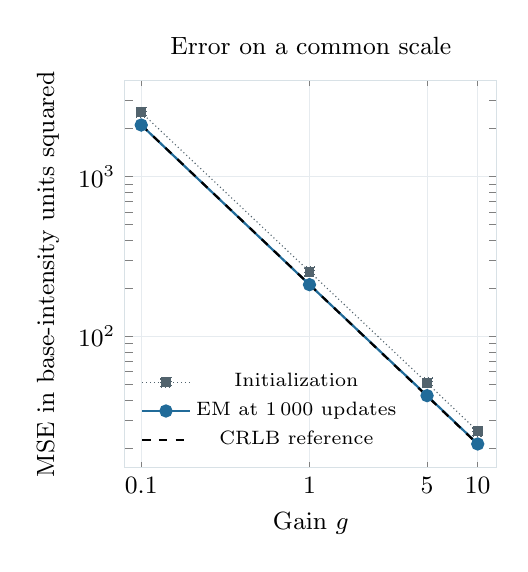
\begin{tikzpicture}
\begin{loglogaxis}[width=.52\linewidth,height=6.5cm,
 xmin=.08,xmax=13,xtick={.1,1,5,10},xticklabels={0.1,1,5,10},
 ymin=15,ymax=4000,xlabel={Gain $g$},ylabel={MSE in base-intensity units squared},
 legend style={at={(0.02,0.02)},anchor=south west,font=\scriptsize},
 title={\small Error on a common scale}]
\addplot[muted,densely dotted,mark=square*,mark size=1.8pt] coordinates {(0.1,2527.6366812578) (1,254.2977156828) (5,51.0404293049) (10,25.4087831948)};
\addlegendentry{Initialization}
\addplot[blue,thick,mark=*,mark size=2pt] coordinates {(0.1,2106.7221724054) (1,210.6570474613) (5,42.4933091754) (10,21.1636207321)};
\addlegendentry{EM at 1\,000 updates}
\addplot[black,dashed,thick] coordinates {(0.1,2110.1969390431) (1,211.0196939043) (5,42.2039387809) (10,21.1019693904)};
\addlegendentry{CRLB reference}
\end{loglogaxis}
\end{tikzpicture}\hfill
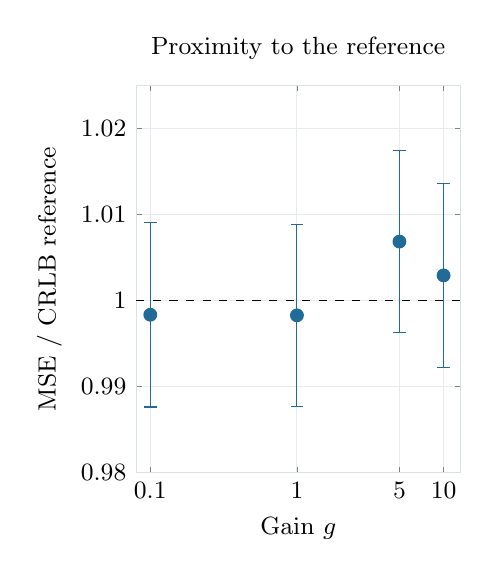
\begin{tikzpicture}
\begin{semilogxaxis}[width=.47\linewidth,height=6.5cm,
 xmin=.08,xmax=13,xtick={.1,1,5,10},xticklabels={0.1,1,5,10},
 ymin=.98,ymax=1.025,ytick={.98,.99,1,1.01,1.02},
 scaled y ticks=false,yticklabel style={/pgf/number format/fixed,/pgf/number format/precision=2},
 xlabel={Gain $g$},ylabel={MSE / CRLB reference},
 title={\small Proximity to the reference}]
\addplot[black,dashed] coordinates {(.08,1) (13,1)};
\addplot[blue,only marks,mark=*,mark size=2.3pt,error bars/.cd,y dir=both,y explicit]
 coordinates {(0.1,0.9983533449) +- (0,0.0107172618) (1,0.9982814569) +- (0,0.0105690744) (5,1.0068564784) +- (0,0.0106040835) (10,1.0029215918) +- (0,0.0107124082)};
\end{semilogxaxis}
\end{tikzpicture}
\caption{Left: gain-normalized estimation error and true-parameter CRLB. Both axes are logarithmic. Right: EM-to-CRLB ratios with approximate 95\% Monte Carlo intervals; the vertical axis is deliberately focused around one. Each point uses 10\,000 independent trials. Line segments on the left connect the four tested gains.}
\label{fig:gain}
\end{figure}

\begin{table}[H]\small
\caption{Final error after 1\,000 updates. MSE and CRLB are divided by $g^2$; intervals describe uncertainty in the Monte Carlo mean.}
\begin{tabularx}{\linewidth}{@{}r r >{\centering\arraybackslash}X r r@{}}\toprule
Gain & MSE & 95\% MC interval & CRLB & Ratio\\\midrule
0.1 & 2,106.72 & [2,084.11, 2,129.34] & 2,110.20 & 0.9984\\
1 & 210.66 & [208.43, 212.89] & 211.02 & 0.9983\\
5 & 42.49 & [42.05, 42.94] & 42.20 & 1.0069\\
10 & 21.16 & [20.94, 21.39] & 21.10 & 1.0029\\
\bottomrule\end{tabularx}
\end{table}

\subsection*{Reading the comparison correctly}
Equation~\eqref{eq:gain} predicts a reference proportional to $1/g$, and the simulation follows that scale. The slight excursions above and below the CRLB are smaller than the reported simulation uncertainty. They do not establish finite-sample efficiency or violate the bound: unbiasedness has not been proved for this constrained estimator.

The comparison holds the matrix and base field fixed. It measures the effect of gain for this particular nine-parameter design; it does not average over different anatomies, sensing geometries, or scanner noise mechanisms. The script also records the empirical bias--variance decomposition to make that distinction inspectable.
% RESULTS_END

% CONVERGENCE_START
\sectionpage{Likelihood ascent and reconstruction error}{sec:convergence}
The first trial at $g=1$ makes the difference between optimization and estimation visible. Its exact log likelihood rises from $-68.837$ to $-67.373$. Its MSE initially increases before falling from 36.07 at initialization to 33.17 after 1\,000 updates. The data fit improves monotonically; the error to the true field does not.

\begin{figure}[H]
\centering
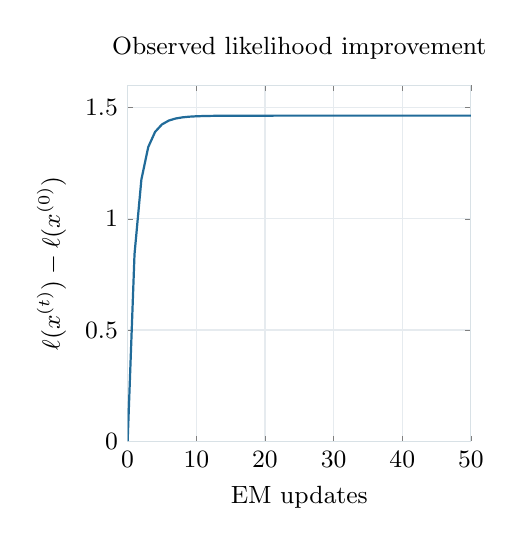
\begin{tikzpicture}
\begin{axis}[width=.49\linewidth,height=6.1cm,
 xmin=0,xmax=50,xtick={0,10,20,30,40,50},ymin=0,ymax=1.6,
 xlabel={EM updates},ylabel={$\ell(x^{(t)})-\ell(x^{(0)})$},
 title={\small Observed likelihood improvement}]
\addplot[blue,thick,no marks] coordinates {(0,0.0000000000) (1,0.8409974796) (2,1.1764293112) (3,1.3228260199) (4,1.3910696154) (5,1.4246753684) (6,1.4420043787) (7,1.4513016253) (8,1.4564676651) (9,1.4594301517) (10,1.4611780649) (11,1.4622359686) (12,1.4628907557) (13,1.4633039249) (14,1.4635689033) (15,1.4637411369) (16,1.4638543125) (17,1.4639293316) (18,1.4639794022) (19,1.4640130026) (20,1.4640356457) (21,1.4640509549) (22,1.4640613317) (23,1.4640683792) (24,1.4640731727) (25,1.4640764370) (26,1.4640786619) (27,1.4640801794) (28,1.4640812150) (29,1.4640819221) (30,1.4640824049) (31,1.4640827348) (32,1.4640829602) (33,1.4640831142) (34,1.4640832194) (35,1.4640832914) (36,1.4640833405) (37,1.4640833742) (38,1.4640833971) (39,1.4640834129) (40,1.4640834236) (41,1.4640834309) (42,1.4640834360) (43,1.4640834394) (44,1.4640834417) (45,1.4640834433) (46,1.4640834444) (47,1.4640834452) (48,1.4640834457) (49,1.4640834461) (50,1.4640834463)};
\end{axis}
\end{tikzpicture}\hfill
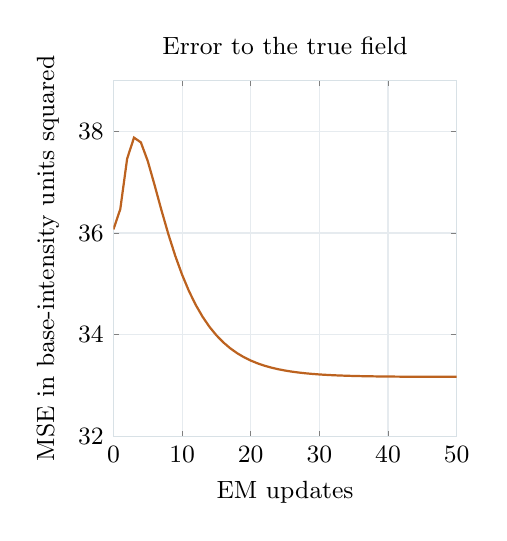
\begin{tikzpicture}
\begin{axis}[width=.49\linewidth,height=6.1cm,
 xmin=0,xmax=50,xtick={0,10,20,30,40,50},ymin=32,ymax=39,
 scaled y ticks=false,xlabel={EM updates},ylabel={MSE in base-intensity units squared},
 title={\small Error to the true field}]
\addplot[orange,thick,no marks] coordinates {(0,36.0704919375) (1,36.4692511630) (2,37.4636911604) (3,37.8771118559) (4,37.7836047052) (5,37.4177832905) (6,36.9424100321) (7,36.4477747271) (8,35.9786455106) (9,35.5545023648) (10,35.1815136165) (11,34.8591383852) (12,34.5836755440) (13,34.3501471967) (14,34.1532817433) (15,33.9880091378) (16,33.8496911650) (17,33.7342083372) (18,33.6379705647) (19,33.5578890269) (20,33.4913301534) (21,33.4360633064) (22,33.3902084397) (23,33.3521869615) (24,33.3206772780) (25,33.2945755097) (26,33.2729613282) (27,33.2550685792) (28,33.2402602298) (29,33.2280071352) (30,33.2178701287) (31,33.2094849698) (32,33.2025497330) (33,33.1968142653) (34,33.1920713910) (35,33.1881495845) (36,33.1849068757) (37,33.1822257842) (38,33.1800091135) (39,33.1781764623) (40,33.1766613307) (41,33.1754087229) (42,33.1743731610) (43,33.1735170409) (44,33.1728092704) (45,33.1722241432) (46,33.1717404064) (47,33.1713404894) (48,33.1710098668) (49,33.1707365299) (50,33.1705105516)};
\end{axis}
\end{tikzpicture}
\caption{One specified trial, not a Monte Carlo average. The first 50 updates are displayed; the full 0--1\,000 trace is saved in \texttt{trace.csv}. The right axis is focused to show the nonmonotonic error. A likelihood plateau alone does not establish exact recovery.}
\end{figure}

\subsection*{Iteration count is not a stopping certificate}
For each trial define $\delta_t=\|x^{(t)}-x^{(t-1)}\|_2/\max(\|x^{(t-1)}\|_2,\varepsilon)$, where $\varepsilon$ is the smallest positive normal floating-point number. At 20 updates, almost no trials satisfy $\delta_t<10^{-6}$. At 200 updates, all trials do, although the average MSE was already close to its final value after 20 updates.
\begin{table}[H]\small
\caption{Fraction of trials meeting the iterate-change threshold and frequency of an invalid unconstrained EM starting point. Each column uses 10\,000 trials per gain.}
\begin{tabularx}{\linewidth}{@{}r >{\centering\arraybackslash}X >{\centering\arraybackslash}X >{\centering\arraybackslash}X@{}}\toprule
Gain & $\delta_{20}<10^{-6}$ & $\delta_{200}<10^{-6}$ & Any negative LS coordinate\\\midrule
0.1 & 0.00\% & 100.00\% & 2.57\%\\
1 & 0.01\% & 100.00\% & 0.00\%\\
5 & 0.15\% & 100.00\% & 0.00\%\\
10 & 0.42\% & 100.00\% & 0.00\%\\
\bottomrule\end{tabularx}
\end{table}

The positivity correction matters at the lowest gain: 2.57\% of least-squares initializations contain a negative coordinate. Clipping makes the initialization valid for multiplicative EM, but is not itself a nonnegative least-squares optimization. Its effect is recorded explicitly in the experiment.

Across 40 million trial-level updates, the largest floating-point likelihood decrease is $1.62\times10^{-10}$, within the stated tolerance $10^{-9}(1+|\ell_{t-1}|)$. This is a numerical check of the implemented update. A small iterate change is a practical diagnostic; a stronger optimization certificate would additionally assess the constrained score conditions.
% CONVERGENCE_END

\sectionpage{Implementation audit and interpretation}{sec:audit}
\subsection*{Reconciling the original report with the repository}
The legacy PDF describes 200 Monte Carlo runs and a gain sweep from 0.1 to 100. The checked-in \texttt{main.m} instead specifies 10\,000 runs, 20 EM updates, and gains $[0.1,1,5,10]$. Its random matrix and base field are not seeded. Consequently, the archived figures cannot be assigned the revised study's conditions or numerical values.

\begin{table}[H]\small
\caption{Material differences addressed in the report supplement. The legacy MATLAB files are retained for provenance.}
\begin{tabularx}{\linewidth}{@{}>{\raggedright\arraybackslash}p{.22\linewidth}>{\raggedright\arraybackslash}X>{\raggedright\arraybackslash}X@{}}\toprule
Issue & Legacy behavior & Controlled study\\\midrule
Forward model & Additive counts described as CT absorption & Linear Poisson intensities distinguished from transmission attenuation\\
Sensing matrix & Predefined matrix overwritten by random rows & Fixed full-rank matrix, printed in full\\
Gain normalization & Division by loop index \texttt{gain\_val\^{}2} & Division by physical gain $g^2$\\
Horizontal axis & Plot receives values only, hence uses indices & Actual gains shown on a numeric logarithmic axis\\
Initialization & Unconstrained inverse normal equations & Least-squares solve followed by a positive floor\\
Information matrix & Evaluated at current estimate $X$ & Evaluated at the known true vector $gb$\\
Log likelihood & Stirling expression includes $0\log0$ & Exact log factorial and explicit zero-count convention\\
Stopping evidence & Fixed 20 updates & Reported checkpoints and relative-change diagnostics\\\bottomrule
\end{tabularx}
\end{table}

\subsection*{What a successful EM run does and does not imply}
The Hessian in Section~\ref{sec:likelihood} is negative semidefinite, so the objective is concave on its valid domain. A constrained stationary solution is globally optimal, but this does not prove that a finite iteration budget has reached it. Strict concavity and uniqueness depend on the informative rows; full rank alone does not make every realized-data Hessian negative definite when counts vanish.

Likelihood ascent measures fit to one noisy count vector. MSE measures distance to a truth that is known only in simulation. A higher likelihood need not reduce MSE, and a nonnegative estimator can have MSE below the ordinary unbiased CRLB through bias. The report therefore treats likelihood, estimation error, and numerical stopping as separate checks.

\subsection*{Scope of the imaging conclusion}
The experiment verifies a small statistical inverse problem. It does not establish diagnostic performance, patient-dose savings, or image quality at clinical resolution. Extensions to transmission CT require the exponential forward model, scanner geometry and calibration, and appropriate treatment of background and electronic noise. At low counts, mixed Poisson--Gaussian modeling can become relevant~\cite{ding}. Regularization and a stopping rule should be evaluated against the intended reconstruction task, rather than inferred from likelihood ascent alone.

\sectionpage{Reproducibility and references}{sec:reproduce}
\subsection*{Reproduce the numerical evidence}
Run the following from the repository root with Python 3 and NumPy. The recorded run uses NumPy 2.3.5. Changing the seed, trial count, iteration budget, or library version may change the last displayed digits or the experiment itself.
\begin{lstlisting}
python3 report/scripts/reproduce.py --trials 10000 \
    --iterations 1000 --seed 20260929
\end{lstlisting}
The script writes \texttt{report/data/results.json}, \texttt{summary.csv}, and \texttt{trace.csv}. The first contains the full design and diagnostics, the second contains gain-by-iteration summary statistics, and the third contains the first gain-one trial at every iteration. Likelihood monotonicity is checked across all trials and updates within a floating-point tolerance. A noiseless fixed-point check and a scalar-versus-vectorized update check exercise the algebra independently.

\subsection*{Edit and build the report}
\texttt{Medical\_Imaging.tex} is a standalone source with embedded vector diagrams and plot coordinates. It opens directly in the built-in LaTeX editor. A conventional TeX environment can also compile it with the packages listed in its preamble. Numerical data are embedded to keep compilation independent of external figure files; after rerunning an altered experiment, update the plotted coordinates and reported values together.

\begin{table}[H]\small
\caption{Files accompanying this edition.}
\begin{tabularx}{\linewidth}{@{}lX@{}}\toprule
File or directory & Role\\\midrule
\texttt{Medical\_Imaging.pdf} & Revised report\\
\texttt{Medical\_Imaging.tex} & Editable source and vector figures\\
\texttt{report/scripts/reproduce.py} & Deterministic simulation and checks\\
\texttt{report/data/} & Numerical results behind the figures\\
\texttt{report/legacy/} & Preserved original Word-exported report\\
\texttt{main.m}, \texttt{EM\_algorithm.m} & Historical MATLAB implementation\\\bottomrule
\end{tabularx}
\end{table}

\begingroup\small\raggedright
\renewcommand{\refname}{References}
\begin{thebibliography}{9}
\bibitem{dempster} A. P. Dempster, N. M. Laird, and D. B. Rubin.
``Maximum likelihood from incomplete data via the EM algorithm.''
\emph{Journal of the Royal Statistical Society, Series B}, 39(1), 1--22, 1977.
\href{https://doi.org/10.1111/j.2517-6161.1977.tb01600.x}{doi:10.1111/j.2517-6161.1977.tb01600.x}.
\bibitem{shepp} L. A. Shepp and Y. Vardi.
``Maximum likelihood reconstruction for emission tomography.''
\emph{IEEE Transactions on Medical Imaging}, 1(2), 113--122, 1982.
\href{https://doi.org/10.1109/TMI.1982.4307558}{doi:10.1109/TMI.1982.4307558}.
\bibitem{miqueles} E. A. Rashed and H. Kudo.
``Towards high-resolution synchrotron radiation imaging with statistical iterative reconstruction.''
\emph{Journal of Synchrotron Radiation}, 20(1), 116--124, 2013.
\href{https://doi.org/10.1107/S0909049512041301}{doi:10.1107/S0909049512041301}.
\bibitem{ding} Q. Ding, Y. Long, X. Zhang, and J. A. Fessler.
``Statistical image reconstruction using mixed Poisson--Gaussian noise model for X-ray CT.''
arXiv:1801.09533, 2018.
\href{https://arxiv.org/abs/1801.09533}{arxiv.org/abs/1801.09533}.
\end{thebibliography}
\endgroup
\end{document}
